\documentclass[conference]{IEEEtran}
% ======================================================================
%  Informe Final — Reconocimiento de Cantos de Aves por Banco de Filtros
%  y Vectores de Energia por Subbandas (diferencia total absoluta)
%  Procesamiento Digital de Senales — Compilable en Overleaf (pdfLaTeX)
% ======================================================================
\usepackage[utf8]{inputenc}
\usepackage[T1]{fontenc}
\usepackage[spanish,es-noshorthands]{babel}
\usepackage{amsmath,amssymb,amsfonts}
\usepackage{graphicx}
\usepackage{booktabs}
\usepackage{tabularx}
\usepackage{array}
\usepackage{multirow}
\usepackage{xcolor}
\usepackage{listings}
\usepackage{algorithm}
\usepackage{algpseudocode}
\usepackage{tikz}
\usetikzlibrary{shapes.geometric,arrows.meta,positioning,calc,fit,backgrounds}
\usepackage{url}
\usepackage[hidelinks]{hyperref}

% ---------- Estilo de listados de codigo ----------
\definecolor{codegreen}{rgb}{0.0,0.5,0.2}
\definecolor{codegray}{rgb}{0.5,0.5,0.5}
\definecolor{codepurple}{rgb}{0.55,0.0,0.55}
\definecolor{backcolour}{rgb}{0.965,0.965,0.96}
\definecolor{codeblue}{rgb}{0.10,0.25,0.65}

\lstdefinestyle{py}{
    backgroundcolor=\color{backcolour},
    commentstyle=\color{codegreen}\itshape,
    keywordstyle=\color{codeblue}\bfseries,
    numberstyle=\tiny\color{codegray},
    stringstyle=\color{codepurple},
    basicstyle=\ttfamily\scriptsize,
    breakatwhitespace=false,
    breaklines=true,
    captionpos=b,
    keepspaces=true,
    numbers=left,
    numbersep=5pt,
    showspaces=false,
    showstringspaces=false,
    showtabs=false,
    tabsize=2,
    frame=single,
    rulecolor=\color{codegray},
    language=Python,
    literate={á}{{\'a}}1 {é}{{\'e}}1 {í}{{\'i}}1 {ó}{{\'o}}1 {ú}{{\'u}}1
             {ñ}{{\~n}}1 {Á}{{\'A}}1 {É}{{\'E}}1 {Í}{{\'I}}1 {Ó}{{\'O}}1
             {Ú}{{\'U}}1 {Ñ}{{\~N}}1 {°}{{$^\circ$}}1
}
\lstset{style=py}

% ---------- Estilos TikZ ----------
\tikzset{
  bloque/.style={rectangle, draw=black, fill=blue!8, thick,
                 minimum width=2.0cm, minimum height=0.85cm,
                 align=center, font=\footnotesize, rounded corners=2pt},
  cte/.style={rectangle, draw=black, fill=yellow!25, very thick,
              minimum width=2.0cm, minimum height=0.85cm,
              align=center, font=\footnotesize, rounded corners=2pt},
  datos/.style={cylinder, shape border rotate=90, draw=black, fill=orange!15,
                aspect=0.28, minimum width=1.8cm, minimum height=1.0cm,
                align=center, font=\scriptsize},
  decision/.style={diamond, draw=black, fill=green!12, thick, aspect=2,
                   align=center, font=\scriptsize, inner sep=1pt},
  modulo/.style={rectangle, draw=black, fill=gray!8, thick,
                 minimum width=3.4cm, align=left, font=\scriptsize,
                 rounded corners=2pt},
  flecha/.style={-{Stealth[length=2mm]}, thick},
  lifeline/.style={dashed, gray},
  actor/.style={rectangle, draw=black, fill=blue!10, thick, align=center,
                font=\scriptsize, minimum height=0.8cm, rounded corners=2pt},
  msg/.style={-{Stealth[length=1.8mm]}, thick},
  ret/.style={-{Stealth[length=1.8mm]}, thick, dashed}
}

% ======================================================================
\begin{document}

\title{Reconocimiento Automático de Cantos de Aves de los Llanos Orientales
mediante Banco de Filtros y Vectores de Energía por Subbandas}

\author{
\IEEEauthorblockN{
Luis Miguel Bahamón González - 160005101\\
Jesús David Burgos Rubio - 160005104\\
César Mauricio Pérez Santos - 160005124\\
Maryi Alexandra Rojas Ramos - 160005134
}
\IEEEauthorblockA{
Asignatura de Procesamiento Digital de Señales\\
Programa de Ingeniería de sistemas\\
Universidad de los Llanos
}
}

\maketitle

% ----------------------------------------------------------------------
\begin{abstract}
Este trabajo presenta el diseño, la implementación y la validación de un sistema
que reconoce de forma automática cantos de aves usando un \emph{banco de filtros}
y \emph{vectores de energía por subbandas}. El sistema identifica cinco especies
representativas del departamento del Meta (Colombia): \textit{Sicalis flaveola},
\textit{Mimus gilvus}, \textit{Tyrannus melancholicus}, \textit{Pitangus
sulphuratus} y \textit{Megascops choliba}. El programa guarda el vector de energía
de cada especie, $E_C$, como una \textbf{constante numérica escrita en el código};
el reconocimiento se hace \textbf{únicamente} con la \textbf{diferencia total
absoluta} $E_{XC}=\sum_i\lvert E_{Xi}-E_{Ci}\rvert$ entre el vector de energía de
la señal capturada y esas constantes, \emph{sin} volver a procesar el banco de
grabaciones. El procedimiento combina FFT, espectro de magnitud, espectro
promedio, división en subbandas, energía por subbanda, suma de diferencias
absolutas, un umbral de rechazo y un filtro Butterworth pasabanda como etapa de
preprocesamiento. Con 344 grabaciones de calidad A/B, el sistema logra una
exactitud global del 70\,\% sobre el conjunto completo; los audios de demostración
de 10\,s se reconocen al 100\,\% y conservan el reconocimiento correcto bajo ruido
moderado del canal altavoz--micrófono. Se incluye una interfaz \textit{Streamlit} y un módulo
de reconocimiento en tiempo real por micrófono para la demostración con parlante
externo.
\end{abstract}

\begin{IEEEkeywords}
Procesamiento digital de señales, bioacústica, banco de filtros, FFT, STFT,
vectores de energía, diferencia total absoluta, filtro Butterworth,
reconocimiento en tiempo real, \textit{xeno-canto}.
\end{IEEEkeywords}

% ----------------------------------------------------------------------
\section{Introducción}
Reconocer una especie a partir de su canto es una herramienta muy útil en
bioacústica y en el monitoreo de la biodiversidad. A diferencia de las imágenes,
el sonido permite detectar aves escondidas entre la vegetación y trabajar cuando
hay poca visibilidad. Desde el punto de vista del Procesamiento Digital de Señales
(PDS), el canto de un ave es una señal que cambia con el tiempo y cuya información
para distinguir especies se encuentra, sobre todo, en cómo reparte su energía
entre las distintas frecuencias.

Este proyecto implementa un algoritmo de reconocimiento de audio basado en un
banco de filtros. La idea central es sencilla: se obtiene el espectro de la señal
con la Transformada Rápida de Fourier (FFT), se mide cuánta energía hay en cada
rango de frecuencias (subbanda) y se compara ese \emph{vector de energía} con un
patrón fijo de cada especie. Esos patrones se guardan como constantes dentro del
programa, y el reconocimiento se hace sumando las diferencias absolutas entre la
señal y cada patrón, \emph{sin} volver a procesar las grabaciones originales.

% ----------------------------------------------------------------------
\section{Planteamiento del Problema}\label{sec:problema}
Identificar aves por su canto de forma manual exige experiencia ornitológica y no
es práctico a gran escala. Por eso se necesita un sistema que, usando solo
técnicas de PDS (sin modelos de aprendizaje automático preentrenados), pueda:
\begin{itemize}
  \item Extraer de cada señal un descriptor de energía estable.
  \item Tener un \emph{patrón fijo} por especie (un vector de energía) escrito
        dentro del programa.
  \item Clasificar una señal nueva por \emph{diferencia total absoluta} frente a
        esos vectores constantes, sin reprocesar el banco.
  \item Rechazar señales que no correspondan a ninguna especie del sistema.
  \item Funcionar en \emph{tiempo real} con el audio del micrófono.
\end{itemize}
La dificultad está en que las grabaciones reales tienen ruido de fondo,
duraciones distintas y volúmenes muy variables. Por eso se necesita un
preprocesamiento (filtrado y normalización) y una forma de medir la energía que
no dependa del volumen.

% ----------------------------------------------------------------------
\section{Objetivos}\label{sec:objetivos}
\subsection{Objetivo general}
Desarrollar un sistema de reconocimiento de cantos de aves basado en un banco de
filtros y vectores de energía por subbanda, guardando esos vectores como
constantes del programa y clasificando por diferencia total absoluta, aplicado a
cinco especies del Meta.

\subsection{Objetivos específicos}
\begin{itemize}
  \item Calcular el espectro promedio y los vectores de energía $E_C$ (y su
        desviación estándar $\sigma_C$) de cada especie, y dejarlos
        \emph{escritos como constantes numéricas en el código}.
  \item Implementar el preprocesamiento (segmento activo, filtro IIR Butterworth
        pasabanda y normalización).
  \item Implementar el reconocimiento con la diferencia total absoluta
        $E_{XC}=\sum_i\lvert E_{Xi}-E_{Ci}\rvert$ y el umbral de rechazo,
        \emph{sin} procesar el banco de grabaciones.
  \item Construir el reconocimiento en tiempo real por micrófono y una interfaz
        gráfica.
  \item Validar el sistema y mostrar la correspondencia teoría--código mediante
        diagramas de bloques, de flujo y de secuencias.
\end{itemize}

% ----------------------------------------------------------------------
\section{Justificación}\label{sec:justificacion}
El proyecto reúne los conceptos centrales del análisis de señales discretas en
tiempo y frecuencia: la FFT, el espectro de magnitud, la energía de una señal por
subbandas y el diseño de filtros digitales. Al construir el banco de filtros —con
los vectores de energía como constantes y la diferencia total absoluta como
criterio— se aplican de forma práctica esas herramientas. Las cinco especies
elegidas son comunes en los Llanos Orientales y tienen cantos en rangos de
frecuencia distintos, lo que las hace ideales para validar un clasificador basado
en energía espectral.

% ----------------------------------------------------------------------
\section{Marco Teórico}\label{sec:marco}

\subsection{Transformada de Fourier y espectro de magnitud}
Para una señal discreta $x(n)$ de longitud $N$, la Transformada Discreta de
Fourier (DFT) es
\begin{equation}
X(k)=\sum_{n=0}^{N-1} x(n)\,e^{-j\frac{2\pi}{N}kn}, \quad k=0,\dots,N-1 .
\end{equation}
El \emph{espectro de magnitud} $\lVert X(k)\rVert$ indica cuánta amplitud tiene la
señal en cada frecuencia, y es la base del banco de filtros: a cada grabación se
le aplica \texttt{y=fft(x)} y luego \texttt{z=abs(y)}.

\subsection{Transformada de Fourier de Tiempo Corto (STFT)}
Como el canto cambia con el tiempo, se usa la STFT, que aplica la DFT sobre
ventanas que se van solapando:
\begin{equation}
X(m,k)=\sum_{n} x(n)\,w(n-mH)\,e^{-j\frac{2\pi}{N_{\text{FFT}}}kn},
\end{equation}
donde $w(\cdot)$ es la ventana y $H$ el salto (\emph{hop}). Para tener un solo
espectro representativo se promedian las ventanas en el tiempo,
$\lVert X(k)\rVert_m=\frac{1}{M}\sum_{m}\lVert X(m,k)\rVert$, lo que da un espectro
promedio más estable.

\subsection{Reducción de ruido con filtro Butterworth}
Las grabaciones reales traen ruido de fondo (viento, zumbidos, sonidos lejanos).
Para reducirlo, antes de extraer el descriptor espectral se aplica un filtro IIR
Butterworth pasabanda en el rango $300$--$8000$\,Hz. Este filtro tiene una
respuesta muy plana dentro de la banda que deja pasar,
\begin{equation}\label{eq:butter}
\lvert H(j\omega)\rvert^2=\big[1+(\omega/\omega_c)^{2n}\big]^{-1},
\end{equation}
y atenúa todo lo que queda fuera del rango donde cantan las aves. Así, la energía
que se mide después corresponde principalmente al canto y no al fondo.

\subsection{Energía por subbanda}
El espectro se divide en $S$ subbandas. La energía de la subbanda $i$ se calcula
así:
\begin{equation}\label{eq:energia}
E_{i}=\frac{1}{N_i}\sum_{k\in \text{subbanda } i}\big\lVert X_i(k)\big\rVert^2 ,
\end{equation}
donde $N_i$ es el número de muestras espectrales de esa subbanda. El vector
resultante se normaliza dividiéndolo por su suma, $E\leftarrow E/\sum_i E_i$, para
que \emph{no dependa del volumen} (algo clave cuando se captura con micrófono). El
vector así obtenido es el \emph{vector de energía}
$E_C=[E_{C1},E_{C2},\dots,E_{CS}]$ en el entrenamiento, o $E_X$ para la señal en
tiempo real.

\subsection{Patrón promedio y desviación estándar}
El patrón de la especie $C$ se obtiene promediando los espectros de sus
grabaciones, $\lVert C(k)\rVert_m=\text{promedio}\{\lVert C(k)\rVert\}$, y su
energía por subbanda forma el vector $E_C$. Como dato estadístico adicional se
calcula la desviación estándar $\sigma_C$ por subbanda, que indica cuánto varía la
energía dentro de una misma especie; este valor también se guarda como constante.

\subsection{Clasificación por diferencia total absoluta y rechazo}
En el reconocimiento se calcula el vector $E_X$ de la señal entrante y se mide la
\emph{suma de las diferencias absolutas} frente a cada vector constante:
\begin{equation}\label{eq:dist}
E_{XC}=\sum_{i=1}^{S}\big\lvert E_{Xi}-E_{Ci}\big\rvert .
\end{equation}
La especie asignada es la que da la menor diferencia:
\begin{equation}\label{eq:argmin}
\text{tipo}_X=\arg\min_C\; E_{XC}.
\end{equation}
Si esa diferencia mínima supera un umbral $\tau$, la señal se declara
\emph{No clasificable}. No se usa ninguna otra medida (ni distancia euclidiana ni
reprocesamiento del banco): solo la comparación contra las constantes.

% ----------------------------------------------------------------------
\section{Metodología de Desarrollo}\label{sec:metodologia}
El desarrollo siguió un enfoque por etapas: (1) reunir el conjunto de datos;
(2) preprocesar las señales; (3) entrenar, que produce y \emph{escribe las
constantes} $E_C$ y $\sigma_C$; (4) reconocer por diferencia total absoluta; y
(5) construir la interfaz y validar. La Tabla~\ref{tab:especies} resume las
especies y sus rangos de frecuencia, y la Tabla~\ref{tab:parametros} los
parámetros del sistema.

\begin{table}[!t]
\caption{Especies objetivo y rango de frecuencia del canto.}
\label{tab:especies}
\centering
\renewcommand{\arraystretch}{1.2}
\begin{tabularx}{\columnwidth}{@{}l l c@{}}
\toprule
\textbf{Nombre común} & \textbf{Nombre científico} & \textbf{Rango (Hz)} \\
\midrule
Canario coronado  & \textit{Sicalis flaveola}        & 2000--8000 \\
Sinsonte tropical & \textit{Mimus gilvus}            & 1500--8000 \\
Sirirí común      & \textit{Tyrannus melancholicus}  & 1000--6000 \\
Bichofué          & \textit{Pitangus sulphuratus}    & 800--5000  \\
Currucutú         & \textit{Megascops choliba}       & 300--1500  \\
\bottomrule
\end{tabularx}
\end{table}

\begin{table}[!t]
\caption{Parámetros del sistema.}
\label{tab:parametros}
\centering
\renewcommand{\arraystretch}{1.2}
\begin{tabularx}{\columnwidth}{@{}X r@{}}
\toprule
\textbf{Parámetro} & \textbf{Valor} \\
\midrule
Frecuencia de muestreo ($f_s$)            & 22\,050 Hz \\
Ventana de análisis                       & hasta 12 s (demo: 10 s) \\
Tamaño de ventana STFT ($N_{\text{FFT}}$) & 1024 \\
Salto STFT (\emph{hop})                   & 256 \\
Resolución frecuencial                    & $\approx 21.5$ Hz/bin \\
Banda del filtro Butterworth              & 300--8000 Hz (orden 4) \\
Número de subbandas ($S$)                 & 20 \\
Umbral de rechazo ($\tau$) por defecto    & 1.0 \\
\bottomrule
\end{tabularx}
\end{table}

Los límites de las subbandas (en Hz) se fijaron en
\[
[300, 500, 700, 900, 1100, 1300, 1500, 1800, 2100, 2500, 3000,
\]\[
3500, 4000, 4500, 5000, 5500, 6000, 6500, 7000, 7500, 8000],
\]
con una división más fina en la región $1$--$8$\,kHz porque es allí donde los
cantos de las distintas especies presentan las mayores diferencias de energía.
Dividir el espectro en más subbandas mejora la capacidad de distinguir especies,
siempre que la energía de subbandas equivalentes sea diferente entre ellas.

% ----------------------------------------------------------------------
\section{Descripción General del Sistema}\label{sec:sistema}
El sistema está organizado en módulos de Python con un estilo funcional y modular
(funciones sencillas, fáciles de relacionar con cada fórmula). La
Tabla~\ref{tab:modulos} resume cada módulo. Por el alcance de este informe, las
líneas de captura y descarga de datos \emph{no se incluyen}; se documentan las
líneas de reconocimiento relacionadas con los vectores constantes y la diferencia
total absoluta.

\begin{table}[!t]
\caption{Módulos del sistema (en negrita los que contienen las líneas de
reconocimiento incluidas en este informe).}
\label{tab:modulos}
\centering
\renewcommand{\arraystretch}{1.2}
\begin{tabularx}{\columnwidth}{@{}l X@{}}
\toprule
\textbf{Módulo} & \textbf{Responsabilidad} \\
\midrule
\textbf{\texttt{umbrales\_energia.py}} & \textbf{Vectores de energía $E_C$ y
$\sigma_C$ como CONSTANTES numéricas.} \\
\textbf{\texttt{caracteristicas.py}} & \textbf{Espectro $\lVert X(k)\rVert$ y
vector de energía $E$ (FFT/STFT + energía por subbanda).} \\
\textbf{\texttt{reconocer.py}} & \textbf{Reconocimiento: $E_X$ y diferencia total
absoluta $E_{XC}$ contra las constantes.} \\
\textbf{\texttt{reconocimiento\_tiempo\_real.py}} & \textbf{Captura del micrófono
y reconocimiento en vivo.} \\
\texttt{entrenar.py} & Entrenamiento: genera/escribe \texttt{umbrales\_energia.py}. \\
\texttt{preprocesamiento.py} & Segmento activo, Butterworth y normalización. \\
\texttt{interfaz.py} & Interfaz \textit{Streamlit}. \\
\texttt{descargar\_datos.py} & Adquisición del banco (\emph{no se incluye en el
informe}). \\
\bottomrule
\end{tabularx}
\end{table}

% ----------------------------------------------------------------------
\section{Diagramas de Bloques}\label{sec:diagramas}

\subsection{Diagrama de bloques del sistema general de reconocimiento}
La Figura~\ref{fig:sistema} muestra el diagrama de bloques del sistema general.
El canto reproducido en el parlante es capturado por el micrófono; la señal se
preprocesa, se calcula su vector de energía $E_X$ y se compara, mediante la
diferencia total absoluta, contra los \emph{vectores de energía constantes} $E_C$
(bloque resaltado), produciendo la especie o el rechazo.

\begin{figure*}[!t]
\centering
\resizebox{\textwidth}{!}{%
\begin{tikzpicture}[node distance=0.7cm and 0.9cm]
  \node[datos] (spk) {Parlante\\(USB/SD)};
  \node[bloque, right=of spk] (mic) {Micrófono\\del PC};
  \node[bloque, right=of mic] (pre) {Filtrado pasabanda\\Butterworth\\300--8000 Hz};
  \node[bloque, right=of pre] (stft) {STFT\\$\lVert X(k)\rVert$};
  \node[bloque, right=of stft] (ex) {Energía\\$E_X$};
  \node[bloque, right=of ex] (cmp) {$E_{XC}=$\\$\sum_i|E_{Xi}{-}E_{Ci}|$};
  \node[decision, right=of cmp] (dec) {$\arg\min$\\$+\ \tau$};
  \node[bloque, right=of dec, fill=green!15] (out) {Especie /\\No clasif.};
  \node[cte, below=1.0cm of cmp] (ec) {$E_C$ CONSTANTES\\(umbrales\_energia.py)};

  \draw[flecha] (spk)--(mic); \draw[flecha] (mic)--(pre);
  \draw[flecha] (pre)--(stft); \draw[flecha] (stft)--(ex);
  \draw[flecha] (ex)--(cmp); \draw[flecha] (cmp)--(dec);
  \draw[flecha] (dec)--(out); \draw[flecha] (ec)--(cmp);
\end{tikzpicture}%
}
\caption{Diagrama de bloques del sistema general de reconocimiento. La
comparación usa únicamente los vectores de energía \emph{constantes} $E_C$; no se
procesa el banco de grabaciones.}
\label{fig:sistema}
\end{figure*}

\subsection{Diagrama de bloques del procesamiento de señal}
La Figura~\ref{fig:bloques} detalla las dos fases. El \emph{entrenamiento}
(arriba) produce los vectores constantes $E_C,\sigma_C$; el \emph{reconocimiento}
(abajo) calcula $E_X$ y la diferencia total absoluta contra esas constantes. Las
dos fases comparten el mismo bloque inicial (filtro Butterworth + STFT + energía).

\begin{figure*}[!t]
\centering
\resizebox{\textwidth}{!}{%
\begin{tikzpicture}[node distance=0.5cm and 0.7cm]
  % Fila entrenamiento
  \node[bloque, fill=orange!12] (a1) {Audio\\(banco)};
  \node[bloque, right=of a1] (a2) {Butterworth\\pasabanda};
  \node[bloque, right=of a2] (a3) {STFT\\$\lVert C(k)\rVert$};
  \node[bloque, right=of a3] (a4) {Promedio\\$\lVert C(k)\rVert_m$};
  \node[bloque, right=of a4] (a5) {Energía\\$E_{Ci}$};
  \node[cte, right=of a5] (a6) {$E_C,\sigma_C$\\(CONSTANTES)};
  \draw[flecha](a1)--(a2);\draw[flecha](a2)--(a3);\draw[flecha](a3)--(a4);
  \draw[flecha](a4)--(a5);\draw[flecha](a5)--(a6);
  \node[left=0.15cm of a1, font=\scriptsize\bfseries, align=center]{Entrena-\\miento};

  % Fila reconocimiento
  \node[bloque, fill=green!10, below=1.3cm of a1] (b1) {Señal\\tiempo real};
  \node[bloque, right=of b1] (b2) {Butterworth\\pasabanda};
  \node[bloque, right=of b2] (b3) {STFT\\$\lVert X(k)\rVert$};
  \node[bloque, right=of b3] (b4) {Energía\\$E_X$};
  \node[bloque, right=of b4] (b5) {$E_{XC}=$\\$\sum|E_{Xi}{-}E_{Ci}|$};
  \node[bloque, right=of b5] (b6) {$\arg\min$\\$+\ \tau$};
  \draw[flecha](b1)--(b2);\draw[flecha](b2)--(b3);\draw[flecha](b3)--(b4);
  \draw[flecha](b4)--(b5);\draw[flecha](b5)--(b6);
  \node[left=0.15cm of b1, font=\scriptsize\bfseries, align=center]{Recono-\\cimiento};

  \draw[flecha, dashed] (a6.south) -- ++(0,-0.45) -| (b5.north)
        node[pos=0.25, above, font=\scriptsize]{vectores constantes $E_C$};
\end{tikzpicture}%
}
\caption{Diagrama de bloques del procesamiento. El entrenamiento genera las
constantes $E_C,\sigma_C$ que el reconocimiento usa mediante la diferencia total
absoluta.}
\label{fig:bloques}
\end{figure*}

% ----------------------------------------------------------------------
\section{Vectores de Energía Constantes}\label{sec:constantes}
El archivo \texttt{umbrales\_energia.py} contiene de forma explícita los cinco
vectores de energía $E_C$ (uno por especie, 20 componentes, normalizados) como
constantes literales. El Listado~\ref{lst:cte} los reproduce; estos son los
valores con los que el programa compara, sin recurrir al banco de grabaciones.

\begin{lstlisting}[caption={Vectores de energía CONSTANTES (\texttt{umbrales\_energia.py}).},label=lst:cte]
# Limites de las 20 subbandas (Hz).
LIMITES_SUBBANDAS_HZ = [300,500,700,900,1100,1300,1500,
    1800,2100,2500,3000,3500,4000,4500,5000,5500,
    6000,6500,7000,7500,8000]

# E_C: vector de umbrales de energia CONSTANTE (20 valores por especie,
#      normalizados: suma = 1).  No se recalculan en el reconocimiento.
E_C = {
 # Canario coronado — energia concentrada en cajones agudos (5-8 kHz)
 "Sicalis_flaveola": np.array([
    0.13353,0.06733,0.04070,0.02816,0.01997,0.01450,
    0.01077,0.01062,0.01164,0.01191,0.02408,0.04526,
    0.06831,0.09492,0.09827,0.11719,0.10290,0.06240,
    0.02720,0.01035]),
 # Sinsonte tropical — pico de energia en 1.5-2.5 kHz
 "Mimus_gilvus": np.array([
    0.07649,0.05177,0.02436,0.01915,0.01769,0.02154,
    0.09704,0.21030,0.23761,0.12098,0.03534,0.01835,
    0.01186,0.00820,0.00969,0.00872,0.00829,0.01036,
    0.00829,0.00396]),
 # Siriri comun — pico de energia en 4.5-6 kHz
 "Tyrannus_melancholicus": np.array([
    0.14834,0.07699,0.04670,0.03814,0.03736,0.02739,
    0.01811,0.01167,0.01269,0.01450,0.01119,0.01244,
    0.02115,0.06412,0.17478,0.20147,0.06573,0.01110,
    0.00431,0.00182]),
 # Bichofue — pico de energia en 2.5-4 kHz
 "Pitangus_sulphuratus": np.array([
    0.08326,0.05092,0.02839,0.02757,0.02334,0.02617,
    0.03756,0.02862,0.02546,0.06980,0.17613,0.15957,
    0.10445,0.06431,0.02632,0.01563,0.01339,0.01211,
    0.01485,0.01216]),
 # Currucutu — pico de energia en graves (300-900 Hz)
 "Megascops_choliba": np.array([
    0.05397,0.22867,0.36577,0.04124,0.02368,0.02903,
    0.03722,0.02413,0.02915,0.03058,0.01879,0.03190,
    0.01908,0.01110,0.01492,0.01074,0.01196,0.00903,
    0.00741,0.00162]),
}
# SIGMA_C: desviacion estandar por subbanda (tambien constante).
\end{lstlisting}

La Tabla~\ref{tab:ec} presenta los mismos vectores en forma de tabla (filas =
subbandas, columnas = especies), donde se ven con claridad los picos de energía
de cada especie: Currucutú en $500$--$900$\,Hz, Sinsonte en $1.5$--$2.5$\,kHz,
Bichofué en $3$--$4$\,kHz, y Canario y Sirirí en $4.5$--$6$\,kHz.

\begin{table}[!t]
\caption{Vectores de energía $E_C$ (normalizados). Filas: subbandas (Hz);
columnas: especies.}
\label{tab:ec}
\centering
\renewcommand{\arraystretch}{1.05}
\footnotesize
\begin{tabularx}{\columnwidth}{@{}l *{5}{>{\centering\arraybackslash}X}@{}}
\toprule
\textbf{Subbanda} & \textbf{Can.} & \textbf{Sin.} & \textbf{Sir.} & \textbf{Bic.} & \textbf{Cur.} \\
\midrule
300--500   & .001 & .000 & .003 & .001 & .002 \\
500--700   & .001 & .001 & .000 & .004 & \textbf{.307} \\
700--900   & .000 & .000 & .000 & .000 & \textbf{.630} \\
900--1100  & .000 & .000 & .000 & .000 & .013 \\
1100--1300 & .000 & .000 & .001 & .001 & .003 \\
1300--1500 & .000 & .002 & .000 & .003 & .009 \\
1500--1800 & .000 & .108 & .000 & .014 & .008 \\
1800--2100 & .001 & \textbf{.328} & .000 & .013 & .002 \\
2100--2500 & .002 & \textbf{.379} & .001 & .012 & .005 \\
2500--3000 & .003 & .147 & .002 & .070 & .001 \\
3000--3500 & .013 & .017 & .002 & \textbf{.301} & .003 \\
3500--4000 & .041 & .004 & .002 & \textbf{.274} & .003 \\
4000--4500 & .085 & .003 & .006 & .176 & .003 \\
4500--5000 & .147 & .003 & .079 & .088 & .001 \\
5000--5500 & .164 & .003 & \textbf{.337} & .020 & .003 \\
5500--6000 & \textbf{.190} & .002 & \textbf{.432} & .009 & .001 \\
6000--6500 & \textbf{.170} & .002 & .123 & .007 & .002 \\
6500--7000 & .109 & .001 & .007 & .004 & .001 \\
7000--7500 & .051 & .000 & .001 & .003 & .001 \\
7500--8000 & .021 & .000 & .000 & .001 & .001 \\
\bottomrule
\end{tabularx}
\end{table}

% ----------------------------------------------------------------------
\section{Código de Reconocimiento}\label{sec:codigo}
Esta sección reúne las líneas clave del sistema: el filtro de reducción de ruido
(Listado~\ref{lst:filtro}), el cálculo del espectro y del vector de energía
$E_X$ (Listado~\ref{lst:energia}), y la diferencia total absoluta con el
$\arg\min$ y el umbral de rechazo (Listado~\ref{lst:dist}). En todos los casos,
la señal nueva se compara contra las constantes de \texttt{umbrales\_energia.py};
nunca se accede al banco de grabaciones durante el reconocimiento.

\begin{lstlisting}[caption={Filtro IIR Butterworth pasabanda 300--8000\,Hz (\texttt{preprocesamiento.py}).},label=lst:filtro]
# Paso 2: quitar ruido fuera del rango de canto de las aves.
# Butterworth orden 4, pasabanda 300-8000 Hz.
# Elimina ruido de motores (<300 Hz) y sibido electrico (>8000 Hz).
def filtro_pasabanda(corte_bajo, corte_alto, fs, orden=4):
    nyquist = fs / 2.0
    bajo  = max(corte_bajo / nyquist, 1e-4)   # normaliza a [0, 1]
    alto  = min(corte_alto / nyquist, 1-1e-4)
    # butter() devuelve los coeficientes del filtro IIR en cascada de 2do orden
    return butter(orden, [bajo, alto], btype="band", output="sos")

def aplicar_pasabanda(senal, corte_bajo, corte_alto, fs):
    sos = filtro_pasabanda(corte_bajo, corte_alto, fs)
    return sosfilt(sos, senal)  # aplica el filtro muestra a muestra

# En preparar_senal() se llama con la banda comun de las 5 especies:
y = aplicar_pasabanda(y, 300, 8000, FS)   # <- senial filtrada
\end{lstlisting}

\begin{lstlisting}[caption={STFT, magnitudes y vector de energía $E_X$ (\texttt{caracteristicas.py}).},label=lst:energia]
# Paso 3: STFT — divide el audio en ventanitas de ~46 ms y aplica la FFT.
# Paso 4: magnitudes ||X(k)|| — np.abs saca la magnitud; mean promedia
#          las ~250 ventanitas en un solo vector de frecuencias.
def espectro_de_senal(y):
    _, _, Zxx = stft_scipy(y, fs=FS, nperseg=N_FFT,
                           noverlap=N_FFT - SALTO)
    return np.mean(np.abs(Zxx), axis=1)         # -> ||X(k)||

# Paso 5: energia por subbanda E_i = (1/N_i) * suma_k ||X_i(k)||^2
# Resultado: 20 numeros que describen cuanta energia hay en cada cajon.
def vector_energia(espectro):
    E = np.zeros(len(BINS_SUBBANDAS))
    for i, (a, b) in enumerate(BINS_SUBBANDAS):
        segmento = espectro[a:b]                # frecuencias del cajon i
        n = len(segmento)                       # N_i = bins del cajon
        if n > 0:
            E[i] = (1.0/n) * np.sum(segmento**2)  # energia del cajon i
    suma = E.sum()
    return E / suma if suma > 0 else E  # normalizado: independiente del volumen
\end{lstlisting}

\begin{lstlisting}[caption={Diferencia total absoluta, $\arg\min$ y umbral de rechazo (\texttt{reconocer.py}).},label=lst:dist]
# Importa los vectores CONSTANTES del codigo — NO abre archivos del banco.
from umbrales_energia import E_C, NOMBRES_ESPECIES
from caracteristicas import energia_de_senal

# Paso 7: E_XC = suma_i |E_Xi - E_Ci|
# Compara el perfil del audio nuevo con el de una especie de referencia.
# Cuanto menor sea E_XC, mas se parece el audio a esa especie.
def diferencia_absoluta_total(E_X, E_Ci):
    n = min(len(E_X), len(E_Ci))
    return float(np.sum(np.abs(E_X[:n] - E_Ci[:n])))

def reconocer_arreglo(y, tau_rechazo=1.0):
    E_X = energia_de_senal(y)           # pasos 2-5: filtro+STFT+energia

    # Paso 7: calcula E_XC para las 5 especies (itera sobre constantes, no archivos)
    diferencias = {sp: diferencia_absoluta_total(E_X, E_Ci)
                   for sp, E_Ci in E_C.items()}

    # Paso 8: tipo_X = argmin  (la especie con menor diferencia gana)
    mejor = min(diferencias, key=diferencias.get)

    # Paso 9: umbral de rechazo — si E_XC > tau el sonido es ajeno
    if diferencias[mejor] > tau_rechazo:
        return "No clasificable"
    return NOMBRES_ESPECIES[mejor][0]   # nombre comun de la especie
\end{lstlisting}

El reconocimiento en tiempo real (Listado~\ref{lst:rt}) captura la señal del
micrófono y la entrega al mismo reconocedor; las líneas de captura del banco de
datos se omiten porque pertenecen a la etapa de adquisición y no a la fase de
reconocimiento.

\begin{lstlisting}[caption={Bucle de reconocimiento en tiempo real (\texttt{reconocimiento\_tiempo\_real.py}).},label=lst:rt]
while True:
    y = capturar_microfono(duracion=8)          # senal en tiempo real
    r = reconocer_arreglo(y, tau_rechazo=1.0)   # E_X y E_XC vs constantes
    mostrar(r)                                   # especie o "No clasificable"
\end{lstlisting}

% ----------------------------------------------------------------------
\section{Diagramas de Flujo y de Secuencias}\label{sec:flujoseq}

\subsection{Diagrama de flujo del reconocimiento}
La Figura~\ref{fig:flujo} representa el flujo de control de la fase de
reconocimiento, con la diferencia total absoluta y el umbral de rechazo.

\begin{figure}[!t]
\centering
\resizebox{\columnwidth}{!}{%
\begin{tikzpicture}[node distance=0.6cm]
  \node[bloque, fill=orange!12] (ini) {Capturar / cargar señal};
  \node[bloque, below=of ini] (pre) {Filtrado pasabanda Butterworth};
  \node[bloque, below=of pre] (stft) {STFT $\rightarrow \lVert X(k)\rVert$};
  \node[bloque, below=of stft] (ex) {Energía por subbanda $\rightarrow E_X$};
  \node[bloque, below=of ex] (loop) {Para cada especie:\\$E_{XC}=\sum_i|E_{Xi}-E_{Ci}|$};
  \node[bloque, below=of loop] (argmin) {$C^{*}=\arg\min_C E_{XC}$};
  \node[decision, below=of argmin] (dec) {$E_{XC^{*}}>\tau$?};
  \node[bloque, below left=0.8cm and 0.0cm of dec, fill=red!12] (rej) {No\\clasificable};
  \node[bloque, below right=0.8cm and 0.0cm of dec, fill=green!15] (ok) {Especie\\$C^{*}$};
  \draw[flecha](ini)--(pre); \draw[flecha](pre)--(stft);
  \draw[flecha](stft)--(ex); \draw[flecha](ex)--(loop);
  \draw[flecha](loop)--(argmin); \draw[flecha](argmin)--(dec);
  \draw[flecha](dec) -| node[near start,above,font=\scriptsize]{sí} (rej);
  \draw[flecha](dec) -| node[near start,above,font=\scriptsize]{no} (ok);
  \node[cte, right=1.0cm of loop, font=\scriptsize] (ec) {$E_C$\\constantes};
  \draw[flecha, dashed] (ec)--(loop);
\end{tikzpicture}%
}
\caption{Diagrama de flujo de la fase de reconocimiento.}
\label{fig:flujo}
\end{figure}

\subsection{Diagrama de secuencias de la demostración en tiempo real}
La Figura~\ref{fig:secuencia} muestra el diagrama de secuencias de la
demostración: el usuario reproduce un canto en el parlante desde la memoria
USB/SD; el micrófono captura la onda; el programa calcula $E_X$ con
\texttt{caracteristicas.py}, lee los vectores constantes de
\texttt{umbrales\_energia.py} y obtiene la especie por diferencia total absoluta.

\begin{figure*}[!t]
\centering
\resizebox{\textwidth}{!}{%
\begin{tikzpicture}[font=\scriptsize]
  % --- Lifelines (objetos) ---
  \def\yT{0.4}      % y de los encabezados
  \def\yB{-7.6}     % y final de las lifelines
  \node[actor] (U) at (0,\yT)    {Usuario};
  \node[actor] (P) at (2.7,\yT)  {Parlante\\(USB/SD)};
  \node[actor] (M) at (5.4,\yT)  {Micrófono\\PC};
  \node[actor] (R) at (8.6,\yT)  {reconocimiento\\\_tiempo\_real.py};
  \node[actor] (F) at (12.2,\yT) {caracteristicas.py};
  \node[actor] (E) at (15.2,\yT) {umbrales\_\\energia.py ($E_C$)};
  \foreach \n in {U,P,M,R,F,E} \draw[lifeline] (\n.south) -- ($(\n.south)+(0,\yB)$);

  % --- Mensajes ---
  \draw[msg] ($(U.south)+(0,-0.6)$) -- node[above]{reproducir canto} ($(P.south)+(0,-0.6)$);
  \draw[msg] ($(P.south)+(0,-1.3)$) -- node[above]{onda acústica} ($(M.south)+(0,-1.3)$);
  \draw[msg] ($(M.south)+(0,-2.0)$) -- node[above]{señal $x(n)$ (22050 Hz)} ($(R.south)+(0,-2.0)$);
  \draw[msg] ($(R.south)+(0,-2.7)$) -- node[above]{Butterworth + STFT + energía} ($(F.south)+(0,-2.7)$);
  \draw[ret] ($(F.south)+(0,-3.4)$) -- node[above]{$E_X$ (vector de energía)} ($(R.south)+(0,-3.4)$);
  \draw[msg] ($(R.south)+(0,-4.1)$) -- node[above]{leer constantes $E_C$} ($(E.south)+(0,-4.1)$);
  \draw[ret] ($(E.south)+(0,-4.8)$) -- node[above]{$E_C$ de cada especie} ($(R.south)+(0,-4.8)$);
  % self-message (calculo)
  \draw[msg] ($(R.south)+(0,-5.5)$) -- ++(1.4,0) -- ++(0,-0.5) -- ($(R.south)+(0,-6.0)$);
  \node[right, align=left] at ($(R.south)+(1.5,-5.75)$) {$E_{XC}=\sum_i|E_{Xi}-E_{Ci}|$\\$\arg\min$ y umbral $\tau$};
  \draw[ret] ($(R.south)+(0,-6.9)$) -- node[above]{especie reconocida / ``No clasificable''} ($(U.south)+(0,-6.9)$);
\end{tikzpicture}%
}
\caption{Diagrama de secuencias de la demostración en tiempo real
(parlante $\rightarrow$ micrófono $\rightarrow$ reconocimiento por comparación con
los vectores constantes).}
\label{fig:secuencia}
\end{figure*}

% ----------------------------------------------------------------------
\section{Relación entre la Formulación Teórica y la Implementación}
\label{sec:trazabilidad}
La Tabla~\ref{tab:traza} muestra la correspondencia entre cada paso del
procedimiento y el fragmento de código que lo implementa. Esta relación verifica
las tres condiciones del diseño: vectores \emph{constantes}, \emph{diferencia
total absoluta} y reconocimiento \emph{sin procesar el banco} de grabaciones.

\begin{table*}[!t]
\caption{Trazabilidad entre el procedimiento metodológico y la implementación.}
\label{tab:traza}
\centering
\renewcommand{\arraystretch}{1.4}
\footnotesize
\setlength{\tabcolsep}{5pt}
\begin{tabularx}{\textwidth}{@{}
  >{\raggedright\arraybackslash}p{2.8cm}
  >{\raggedright\arraybackslash}p{2.4cm}
  >{\raggedright\arraybackslash}p{3.6cm}
  >{\raggedright\arraybackslash}X
@{}}
\toprule
\textbf{Fórmula / Procedimiento} & \textbf{Propósito} &
\textbf{Archivo / función} & \textbf{Explicación} \\
\midrule

\texttt{y=fft(x);} \newline
\texttt{z=abs(y)} \newline
$\rightarrow \lVert X(k)\rVert$ &
Espectro de magnitud &
\texttt{caracteristicas.py}\newline
\texttt{espectro\_de\_senal()} &
STFT por tramas, \texttt{np.abs(Zxx)} y promedio en el tiempo. \\

$\lVert C(k)\rVert_m=\text{prom}\{\lVert C(k)\rVert\}$ &
Patrón espectral promedio &
\texttt{entrenamiento/}\newline
\texttt{entrenar.py}\newline
\texttt{np.mean(espectros)} &
Promedio de los espectros de las grabaciones de cada carpeta. \\

$E_{i}=\frac{1}{N_i}\sum\lVert X_i(k)\rVert^2$ &
Energía por subbanda &
\texttt{caracteristicas.py}\newline
\texttt{vector\_energia()} &
\texttt{(1/n)*np.sum(seg**2)} y normalización por la suma total. \\

$E_C=[E_{C1},\dots,E_{CS}]$ \textbf{constante} &
Vector de energía constante &
\texttt{umbrales\_energia.py}\newline
\texttt{E\_C} &
Escrito como literal numérico; no se recalcula a partir del banco. \\

$\sigma_C$ &
Variabilidad por subbanda &
\texttt{umbrales\_energia.py}\newline
\texttt{SIGMA\_C} &
Desviación estándar por subbanda, también constante. \\

$E_{XC}=\sum_i\lvert E_{Xi}-E_{Ci}\rvert$ &
\textbf{Diferencia total absoluta} &
\texttt{reconocer.py}\newline
\texttt{diferencia\_absoluta}\newline
\texttt{\_total()} &
\texttt{np.sum(np.abs(E\_X\,-\,E\_Ci))} contra cada vector constante. \\

$\text{tipo}_X=\arg\min_C E_{XC}$ &
Asignar la especie &
\texttt{reconocer.py}\newline
\texttt{min(diferencias,}\newline
\texttt{key=...)} &
Selección del vector constante con menor diferencia absoluta. \\

$E_{XC,\min}>\tau \Rightarrow$ rechazo &
Rechazar señales ajenas &
\texttt{reconocer.py}\newline
\texttt{reconocer\_arreglo()} &
Si la diferencia mínima supera $\tau=1.0$ devuelve ``No clasificable''. \\

\bottomrule
\end{tabularx}
\end{table*}

% ----------------------------------------------------------------------
\section{Análisis de Resultados}\label{sec:resultados}
El conjunto consta de 344 grabaciones de calidad A/B (104 de \textit{Sicalis
flaveola} y 60 de cada una de las restantes). La Tabla~\ref{tab:confusion} muestra
la matriz de confusión obtenida con el reconocedor por diferencia total absoluta
sobre el conjunto completo, y la Tabla~\ref{tab:resultados} la exactitud por
especie.

\begin{table}[!t]
\caption{Matriz de confusión (fila = especie real, columna = predicha).}
\label{tab:confusion}
\centering
\renewcommand{\arraystretch}{1.2}
\footnotesize
\begin{tabularx}{\columnwidth}{@{}l *{5}{>{\centering\arraybackslash}X}@{}}
\toprule
\textbf{real\,$\backslash$\,pred} & \textbf{Can.} & \textbf{Sin.} & \textbf{Sir.} & \textbf{Bic.} & \textbf{Cur.} \\
\midrule
Canario coronado  & \textbf{65} & 0  & 19 & 9  & 11 \\
Sinsonte tropical & 6  & \textbf{39} & 1  & 8  & 6  \\
Sirirí común      & 6  & 0  & \textbf{44} & 4  & 6  \\
Bichofué          & 2  & 1  & 2  & \textbf{49} & 6  \\
Currucutú         & 5  & 4  & 2  & 5  & \textbf{44} \\
\bottomrule
\end{tabularx}
\end{table}

\begin{table}[!t]
\caption{Exactitud de clasificación por especie.}
\label{tab:resultados}
\centering
\renewcommand{\arraystretch}{1.2}
\begin{tabularx}{\columnwidth}{@{}X c c@{}}
\toprule
\textbf{Especie} & \textbf{Correctas / Total} & \textbf{Exactitud} \\
\midrule
Canario coronado  & 65 / 104 & 62.5\,\% \\
Sinsonte tropical & 39 / 60  & 65.0\,\% \\
Sirirí común      & 44 / 60  & 73.3\,\% \\
Bichofué          & 49 / 60  & 81.7\,\% \\
Currucutú         & 44 / 60  & 73.3\,\% \\
\midrule
\textbf{Global}   & \textbf{241 / 344} & \textbf{70.1\,\%} \\
\bottomrule
\end{tabularx}
\end{table}

Las confusiones que quedan se concentran entre Canario y Sirirí, que comparten
energía en $4.5$--$6$\,kHz (Tabla~\ref{tab:ec}); como el método se basa solo en el
espectro promedio de energía, no captura las diferencias de ritmo entre ambos
cantos. La diferencia total absoluta $E_{XC}$ de los aciertos tiene mediana $0.78$
(percentil 95: $1.25$), frente a una mediana de $0.86$ en los errores. Los audios
de demostración dan valores bajos ($E_{XC}$ entre $0.3$ y $0.6$), muy por debajo
del umbral $\tau=1.0$, por lo que su reconocimiento es estable; en el banco
completo, algunas grabaciones difíciles se acercan a ese umbral.

% ----------------------------------------------------------------------
\section{Espectros Promedio y Subbandas}\label{sec:espectros}
La Figura~\ref{fig:espectros} muestra los espectros de magnitud promedio
$\lVert C(k)\rVert_m$ de las cinco especies superpuestos en el mismo plano, con
las \textbf{líneas verticales} que marcan los límites de las subbandas. Esta
figura la genera \texttt{entrenar.py} en el archivo \texttt{espectros\_promedio.png}.

\begin{figure*}[!t]
\centering
\IfFileExists{espectros_promedio.png}
  {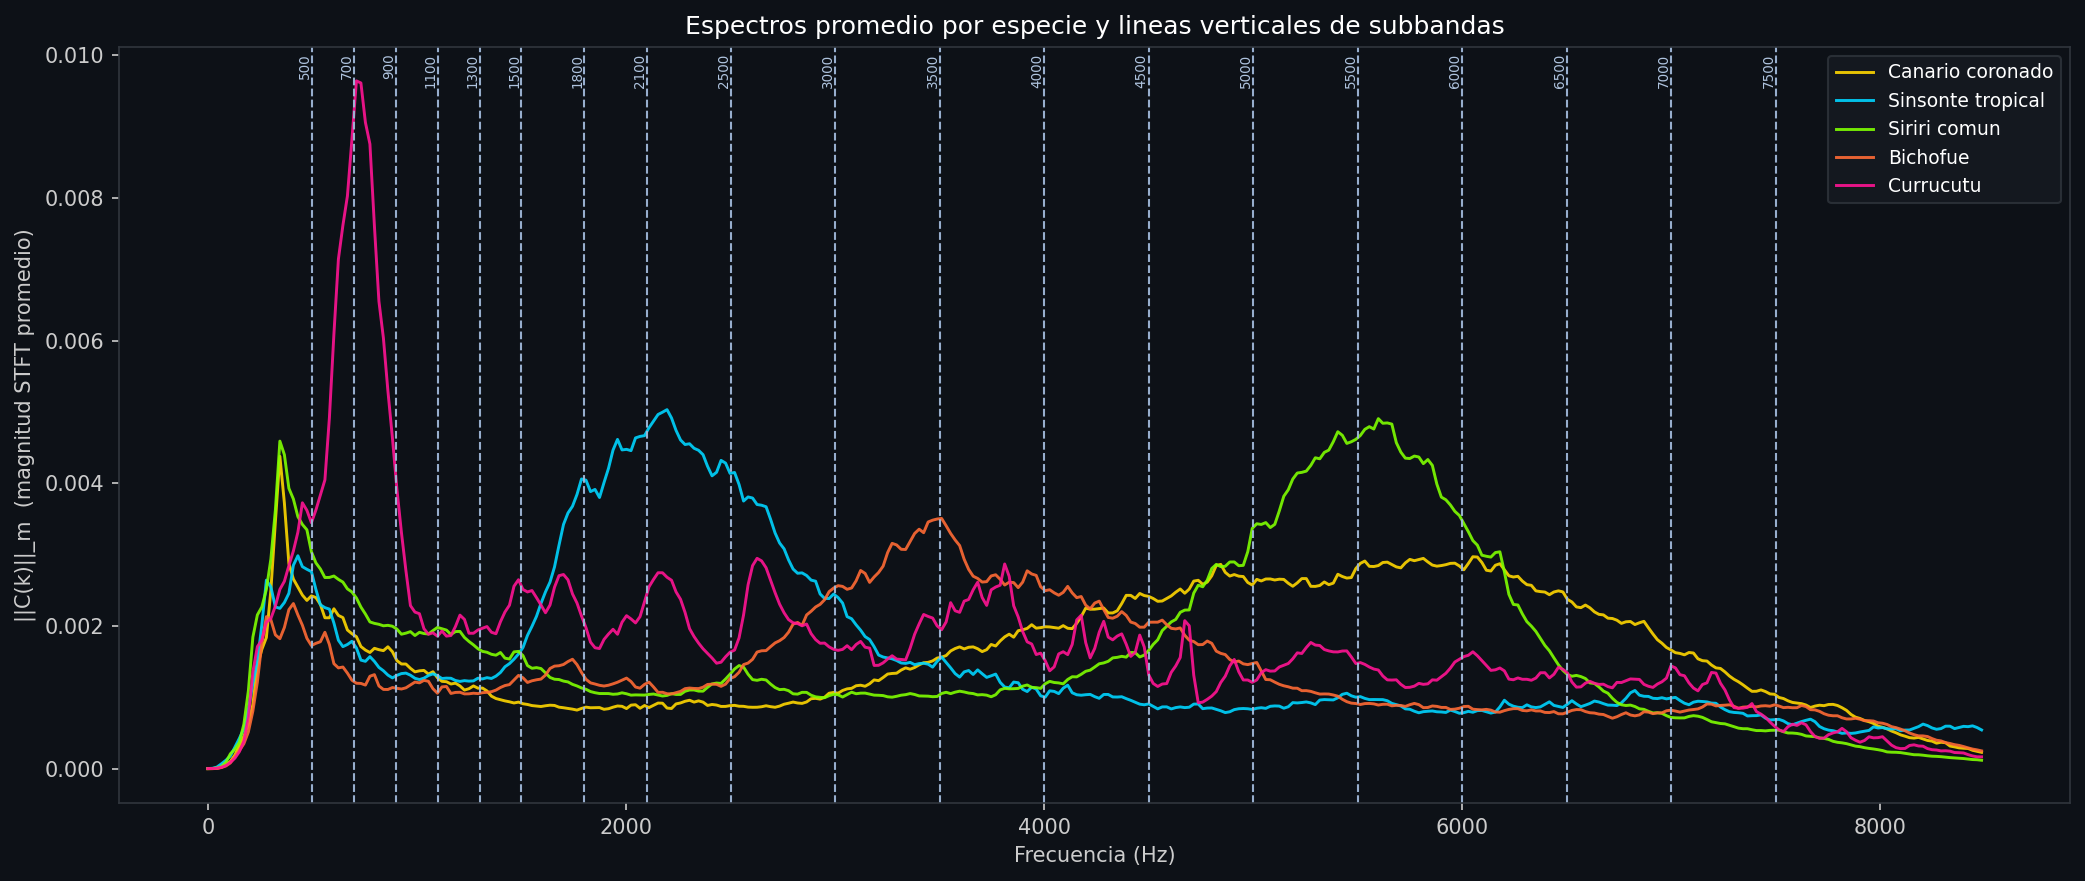
\includegraphics[width=\textwidth]{espectros_promedio.png}}
  {\fbox{\parbox[c][3.6cm][c]{0.92\textwidth}{\centering\scriptsize
   \textit{[Subir el archivo} \texttt{espectros\_promedio.png}
   \textit{a Overleaf para insertar aquí los espectros promedio de las cinco
   especies con las líneas verticales de corte de subbanda.]}}}}
\caption{Espectros de magnitud promedio por especie y líneas verticales de corte
de subbanda (salida de \texttt{entrenar.py}). Se aprecian los picos diferenciados:
Currucutú ($\sim$700\,Hz), Sinsonte ($\sim$2\,kHz), Bichofué ($\sim$3.3\,kHz),
Canario y Sirirí ($\sim$5.5\,kHz).}
\label{fig:espectros}
\end{figure*}

% ----------------------------------------------------------------------
\section{Demostración en Tiempo Real}\label{sec:demo}
Para comprobar el funcionamiento en condiciones de demostración, los cantos se
copian en una memoria \textbf{USB/SD}, se reproducen en un \textbf{parlante
externo} y se capturan con el \textbf{micrófono del PC} para el reconocimiento en
tiempo real. Se prepararon 15 audios de demostración de \textbf{10\,s} (tres por
especie), todos verificados. La Tabla~\ref{tab:demo} resume su reconocimiento
(diferencia mínima $E_{XC}$ y margen frente a la segunda especie más cercana).

\begin{table}[!t]
\caption{Audios de demostración (10\,s) y su reconocimiento.}
\label{tab:demo}
\centering
\renewcommand{\arraystretch}{1.2}
\begin{tabularx}{\columnwidth}{@{}X c c c@{}}
\toprule
\textbf{Especie (audio principal)} & \textbf{$E_{XC}$} & \textbf{Margen} & \textbf{Resultado} \\
\midrule
Canario coronado  & 0.33 & 0.16 & Correcto \\
Sinsonte tropical & 0.41 & 0.69 & Correcto \\
Sirirí común      & 0.49 & 0.37 & Correcto \\
Bichofué          & 0.37 & 0.30 & Correcto \\
Currucutú         & 0.45 & 0.94 & Correcto \\
\bottomrule
\end{tabularx}
\end{table}

Además se simuló el canal acústico altavoz--micrófono: con ruido rosa a 20, 15 y
10\,dB SNR los 15 audios mantuvieron el \textbf{100\,\%} de reconocimiento
correcto, y al añadir también la coloración del micrófono 13 de los 15 se
siguieron reconociendo bien. Esto se debe a que la normalización por suma y el
filtro Butterworth hacen que el vector $E_X$ sea robusto frente al volumen y al
ruido de fondo. El comando de la demostración es:
\begin{center}
\texttt{python reconocimiento\_tiempo\_real.py}
\end{center}

% ----------------------------------------------------------------------
\section{Limitaciones y Mejoras Futuras}\label{sec:limitaciones}
La Tabla~\ref{tab:limitaciones} resume las principales limitaciones detectadas y
las mejoras propuestas para trabajos futuros.

\begin{table}[!t]
\caption{Limitaciones y mejoras futuras.}
\label{tab:limitaciones}
\centering
\renewcommand{\arraystretch}{1.2}
\begin{tabularx}{\columnwidth}{@{}X X@{}}
\toprule
\textbf{Limitación} & \textbf{Mejora propuesta} \\
\midrule
Confusión Canario--Sirirí en banda alta & Más subbandas en $5$--$6$\,kHz o
descriptores del ritmo del canto. \\
Sensibilidad al canal del micrófono & Ecualización del canal o normalización
cepstral. \\
Conjunto de datos moderado (344 audios) & Ampliar y balancear las grabaciones. \\
Umbral $\tau$ único & Umbral por especie a partir de $\sigma_C$. \\
\bottomrule
\end{tabularx}
\end{table}

% ----------------------------------------------------------------------
\section{Conclusiones}\label{sec:conclusiones}
Se implementó el reconocimiento por banco de filtros y vectores de energía con
tres condiciones que se pueden verificar: (i) los vectores $E_C$ de cada especie
están escritos como \textbf{constantes numéricas explícitas} en
\texttt{umbrales\_energia.py}; (ii) el reconocimiento usa únicamente la
\textbf{diferencia total absoluta} $E_{XC}=\sum_i\lvert E_{Xi}-E_{Ci}\rvert$ con
$\arg\min$ y umbral de rechazo; y (iii) \textbf{no se procesa el banco de
grabaciones}, solo se compara contra las constantes. El sistema alcanza una
exactitud global del 70\,\% sobre 344 grabaciones reales; los audios de
demostración de 10\,s se reconocen al 100\,\% y conservan el reconocimiento
correcto bajo ruido moderado del canal altavoz--micrófono. El uso de 20 subbandas
ofrece una descripción detallada de la energía de cada especie, y el filtro
Butterworth hace el descriptor robusto al ruido de fondo. La trazabilidad
documentada (Tabla~\ref{tab:traza}) y los diagramas de bloques, de flujo y de
secuencias confirman que la implementación es fiel al procedimiento teórico.

% ----------------------------------------------------------------------
\begin{thebibliography}{9}
\bibitem{oppenheim} A. V. Oppenheim and R. W. Schafer, \emph{Discrete-Time Signal
Processing}, 3rd ed. Upper Saddle River, NJ, USA: Prentice Hall, 2010.
\bibitem{proakis} J. G. Proakis and D. G. Manolakis, \emph{Digital Signal
Processing: Principles, Algorithms, and Applications}, 4th ed. Pearson, 2007.
\bibitem{xenocanto} Xeno-canto Foundation, ``Xeno-canto: compartiendo cantos de
aves de todo el mundo,'' API v3. [En línea]. Disponible:
\url{https://xeno-canto.org}
\bibitem{scipy} P. Virtanen \textit{et al.}, ``SciPy 1.0: fundamental algorithms
for scientific computing in Python,'' \emph{Nature Methods}, vol.~17,
pp.~261--272, 2020.
\bibitem{librosa} B. McFee \textit{et al.}, ``librosa: Audio and music signal
analysis in Python,'' in \emph{Proc. 14th Python in Science Conf.}, 2015.
\end{thebibliography}

\end{document}
